\chapter{Streamlining the Evaluation of Gesture Recognizers} \label{chap:quantumleap-testing}

Evaluating the performance and efficiency of gesture recognizers is an important step both in the design of gesture-based interfaces, to select the most appropriate gesture recognition algorithm for a specific application (Section~\ref{sec:lui:development-method:implementation}), and in the development of new sensors, signal processing techniques, or gesture recognition algorithms, to compare them against the current state of the art or to assess how they perform in a particular context (Chapter~\ref{chap:radar-experiments}). This chapter thus attempts to answer the following research question, defined in Section~\ref{sec:introduction:research:research-questions}:
%
\begin{itemize}
  \item [RQ5] \textit{How can tools and methods aid in designing gesture-based applications that operate independently of gesture recognition logic?}
\end{itemize}
%
With this objective in mind, this chapter introduces the \ql testing tool, an extension of \ql (Chapter~\ref{chap:quantumleap}) that takes advantage of its standardized modules to provide a simple yet efficient way for researchers and practitioners to evaluate and compare gesture recognition algorithms. This tool facilitates the sharing of testing procedures and their results, thus opening the door for future attempts to reproduce or replicate them.
%
As such, it was used extensively in this thesis, in some of our publications~\cite{Sluyters:2022:LUI,Sluyters:2022:IUI,Sluyters:2023}, and by master's students in their theses~\cite{Neuville:2021,Steeman:2022,Lahousse:2022,Cornet:2023,Giot:2023}. \fig~\ref{fig:quantumleap-testing:graphical-summary} illustrates the main contribution of this chapter and how it fits with the rest of this thesis.

\begin{figure}
  \centering
  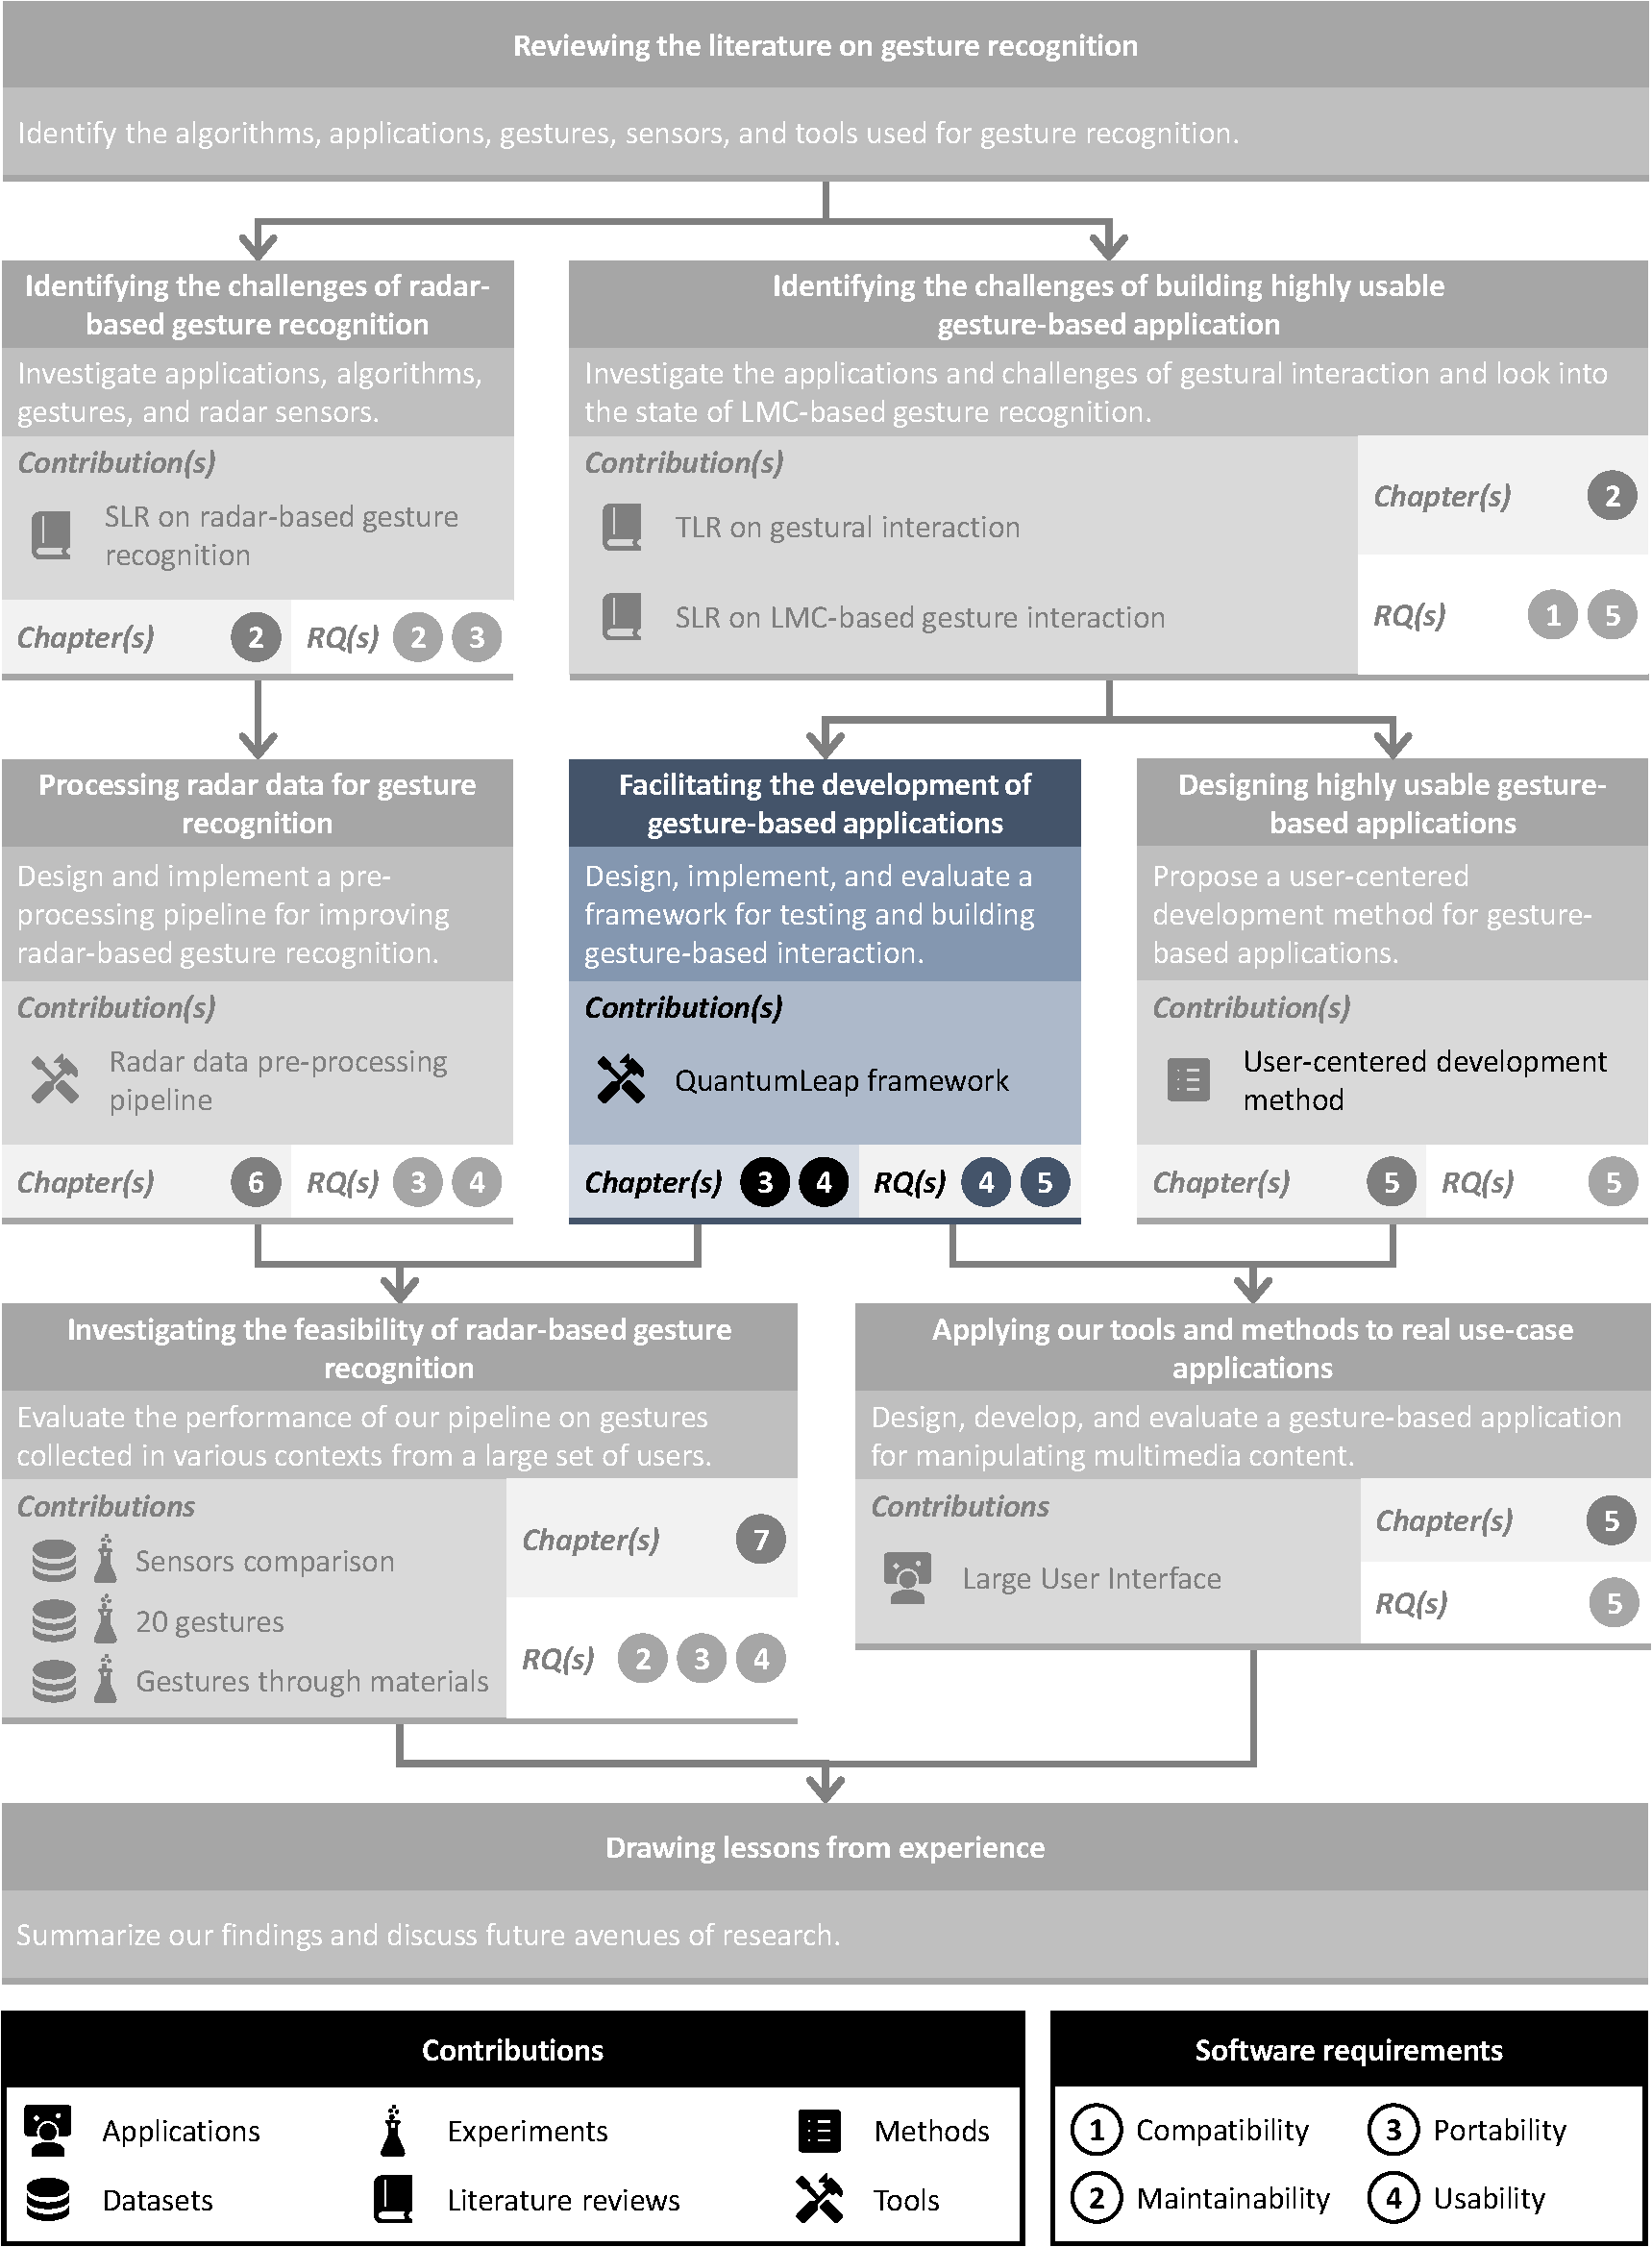
\includegraphics[width=\linewidth]{Figures/QuantumLeap/graphical-summary-quantumleap.pdf}
  \vspace{-18pt}
  \caption{Main contributions of this chapter.}
  \label{fig:quantumleap-testing:graphical-summary}
\end{figure}

The rest of this chapter is divided into three sections.
Section~\ref{sec:quantumleap-testing:description} first explains how the testing tool was integrated into \ql, its main features, and how it can be used to evaluate gesture recognition algorithms.
Section~\ref{sec:quantumleap-testing:discussion} then discusses its main advantages and limitations and Section~\ref{sec:quantumleap-testing:conclusion} concludes this chapter.

\paragraph{Resources.} The \ql testing tool is available on GitHub at \url{https://github.com/sluyters/QuantumLeap}.

%================================================================================%
\section{A Tool for Evaluating Gesture Recognition Algorithms} \label{sec:quantumleap-testing:description}
The \ql testing tool is based on the same architecture as the gesture recognition dataflow and is thus also written in JavaScript (ECMAScript 2019). The reuse of many \ql software components, from its backend to its frontend, vastly simplified its development and allowed this tool to work directly with all of the existing recognizer and dataset modules. \fig~\ref{fig:quantumleap-testing:archi} illustrates the testing tool architecture and data structures for inter-module communication are described in \tab~\ref{tbl:quantumleap:communication-data-structures}.
%
The rest of this section discusses the integration of this tool into \ql and the various testing procedures that it supports.

\begin{figure}[t]
  \centering
  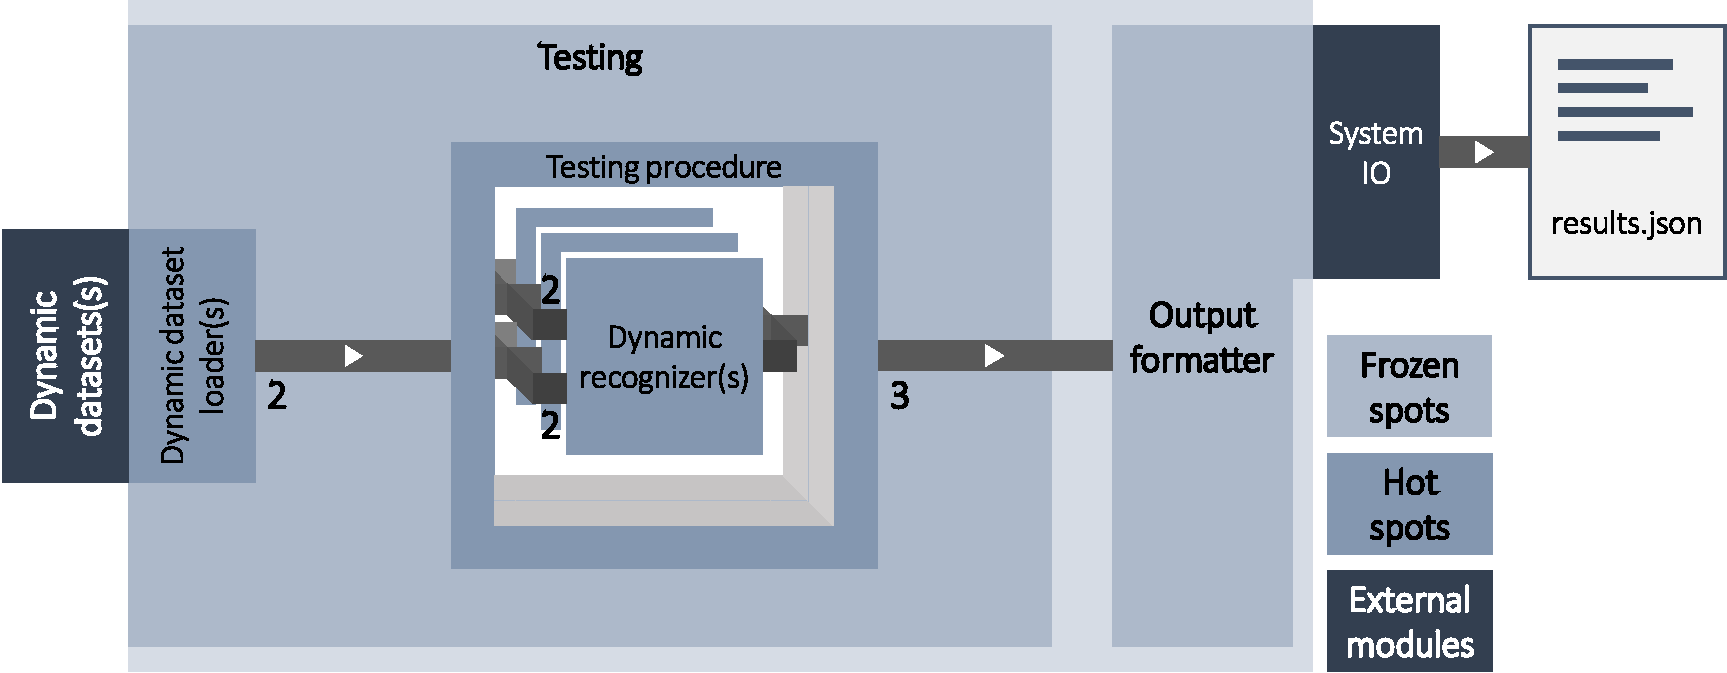
\includegraphics[width=\linewidth]{Figures/QuantumLeapTesting/quantumleap-testing.pdf}
  \vspace{-8pt}
  \caption{\ql testing tool architecture.}
  % \vspace{-8pt}
  \label{fig:quantumleap-testing:archi}
\end{figure}

%--------------------------------------------------------------------------------%
\subsection{Integration into \ql} \label{sec:quantumleap-testing:description:ql-integration}
\subsubsection{Modules} \label{sec:quantumleap-testing:description:ql-integration:modules}
This tool relies on the same dataset and recognizer modules as the \ql gesture recognition dataflow. However, it only supports the testing of static and dynamic recognizers. Testing other types of modules (\eg a segmenter) or combinations of modules (\eg a segmenter and a dynamic recognizer) would require modifications to its source code.

\subsubsection{Configuration} \label{sec:quantumleap-testing:description:ql-integration:configuration}

\begin{figure}[bt]
  \centering
  \begin{subfigure}{.49\textwidth}
      \centering
      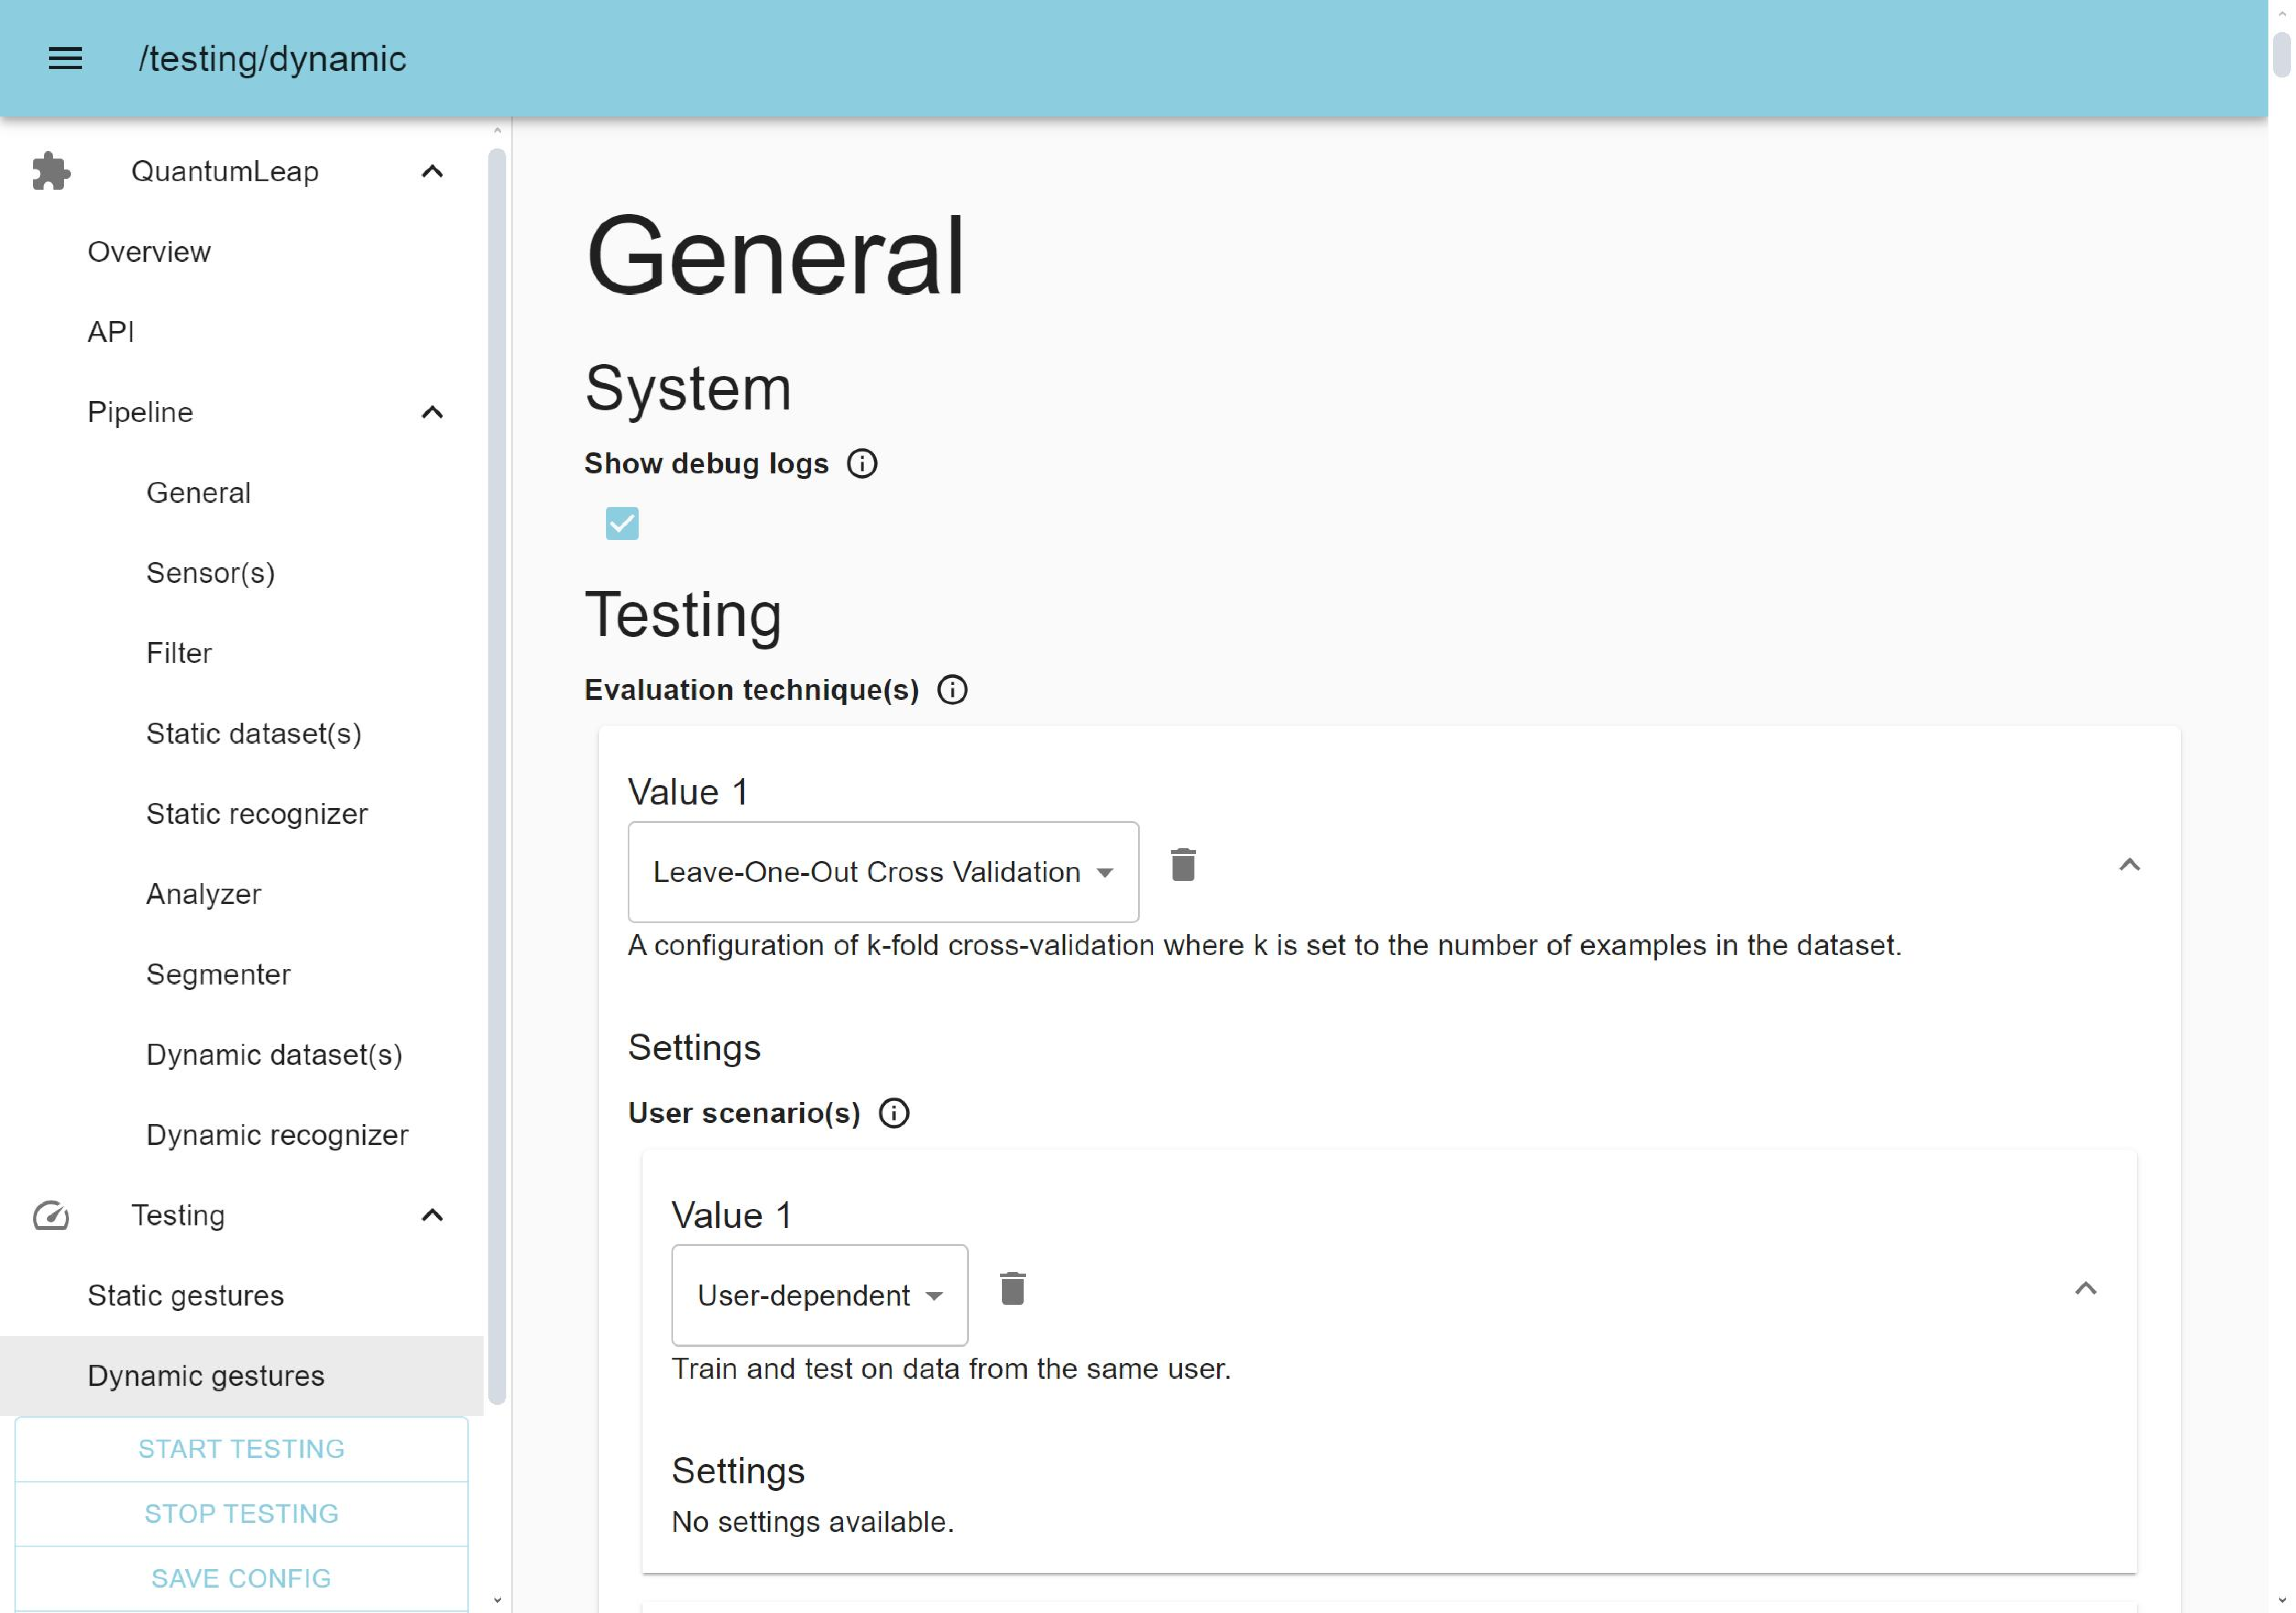
\includegraphics[width=\linewidth]{Figures/QuantumLeapTesting/QL-Testing-EvaluationTechnique.pdf}  
      \vspace{-15pt}
      \captionsetup{width=.9\linewidth}
      \caption{Evaluation techniques.}
      \label{fig:quantumleap-testing:ui:1}
  \end{subfigure}
  \begin{subfigure}{.49\textwidth}
      \centering
      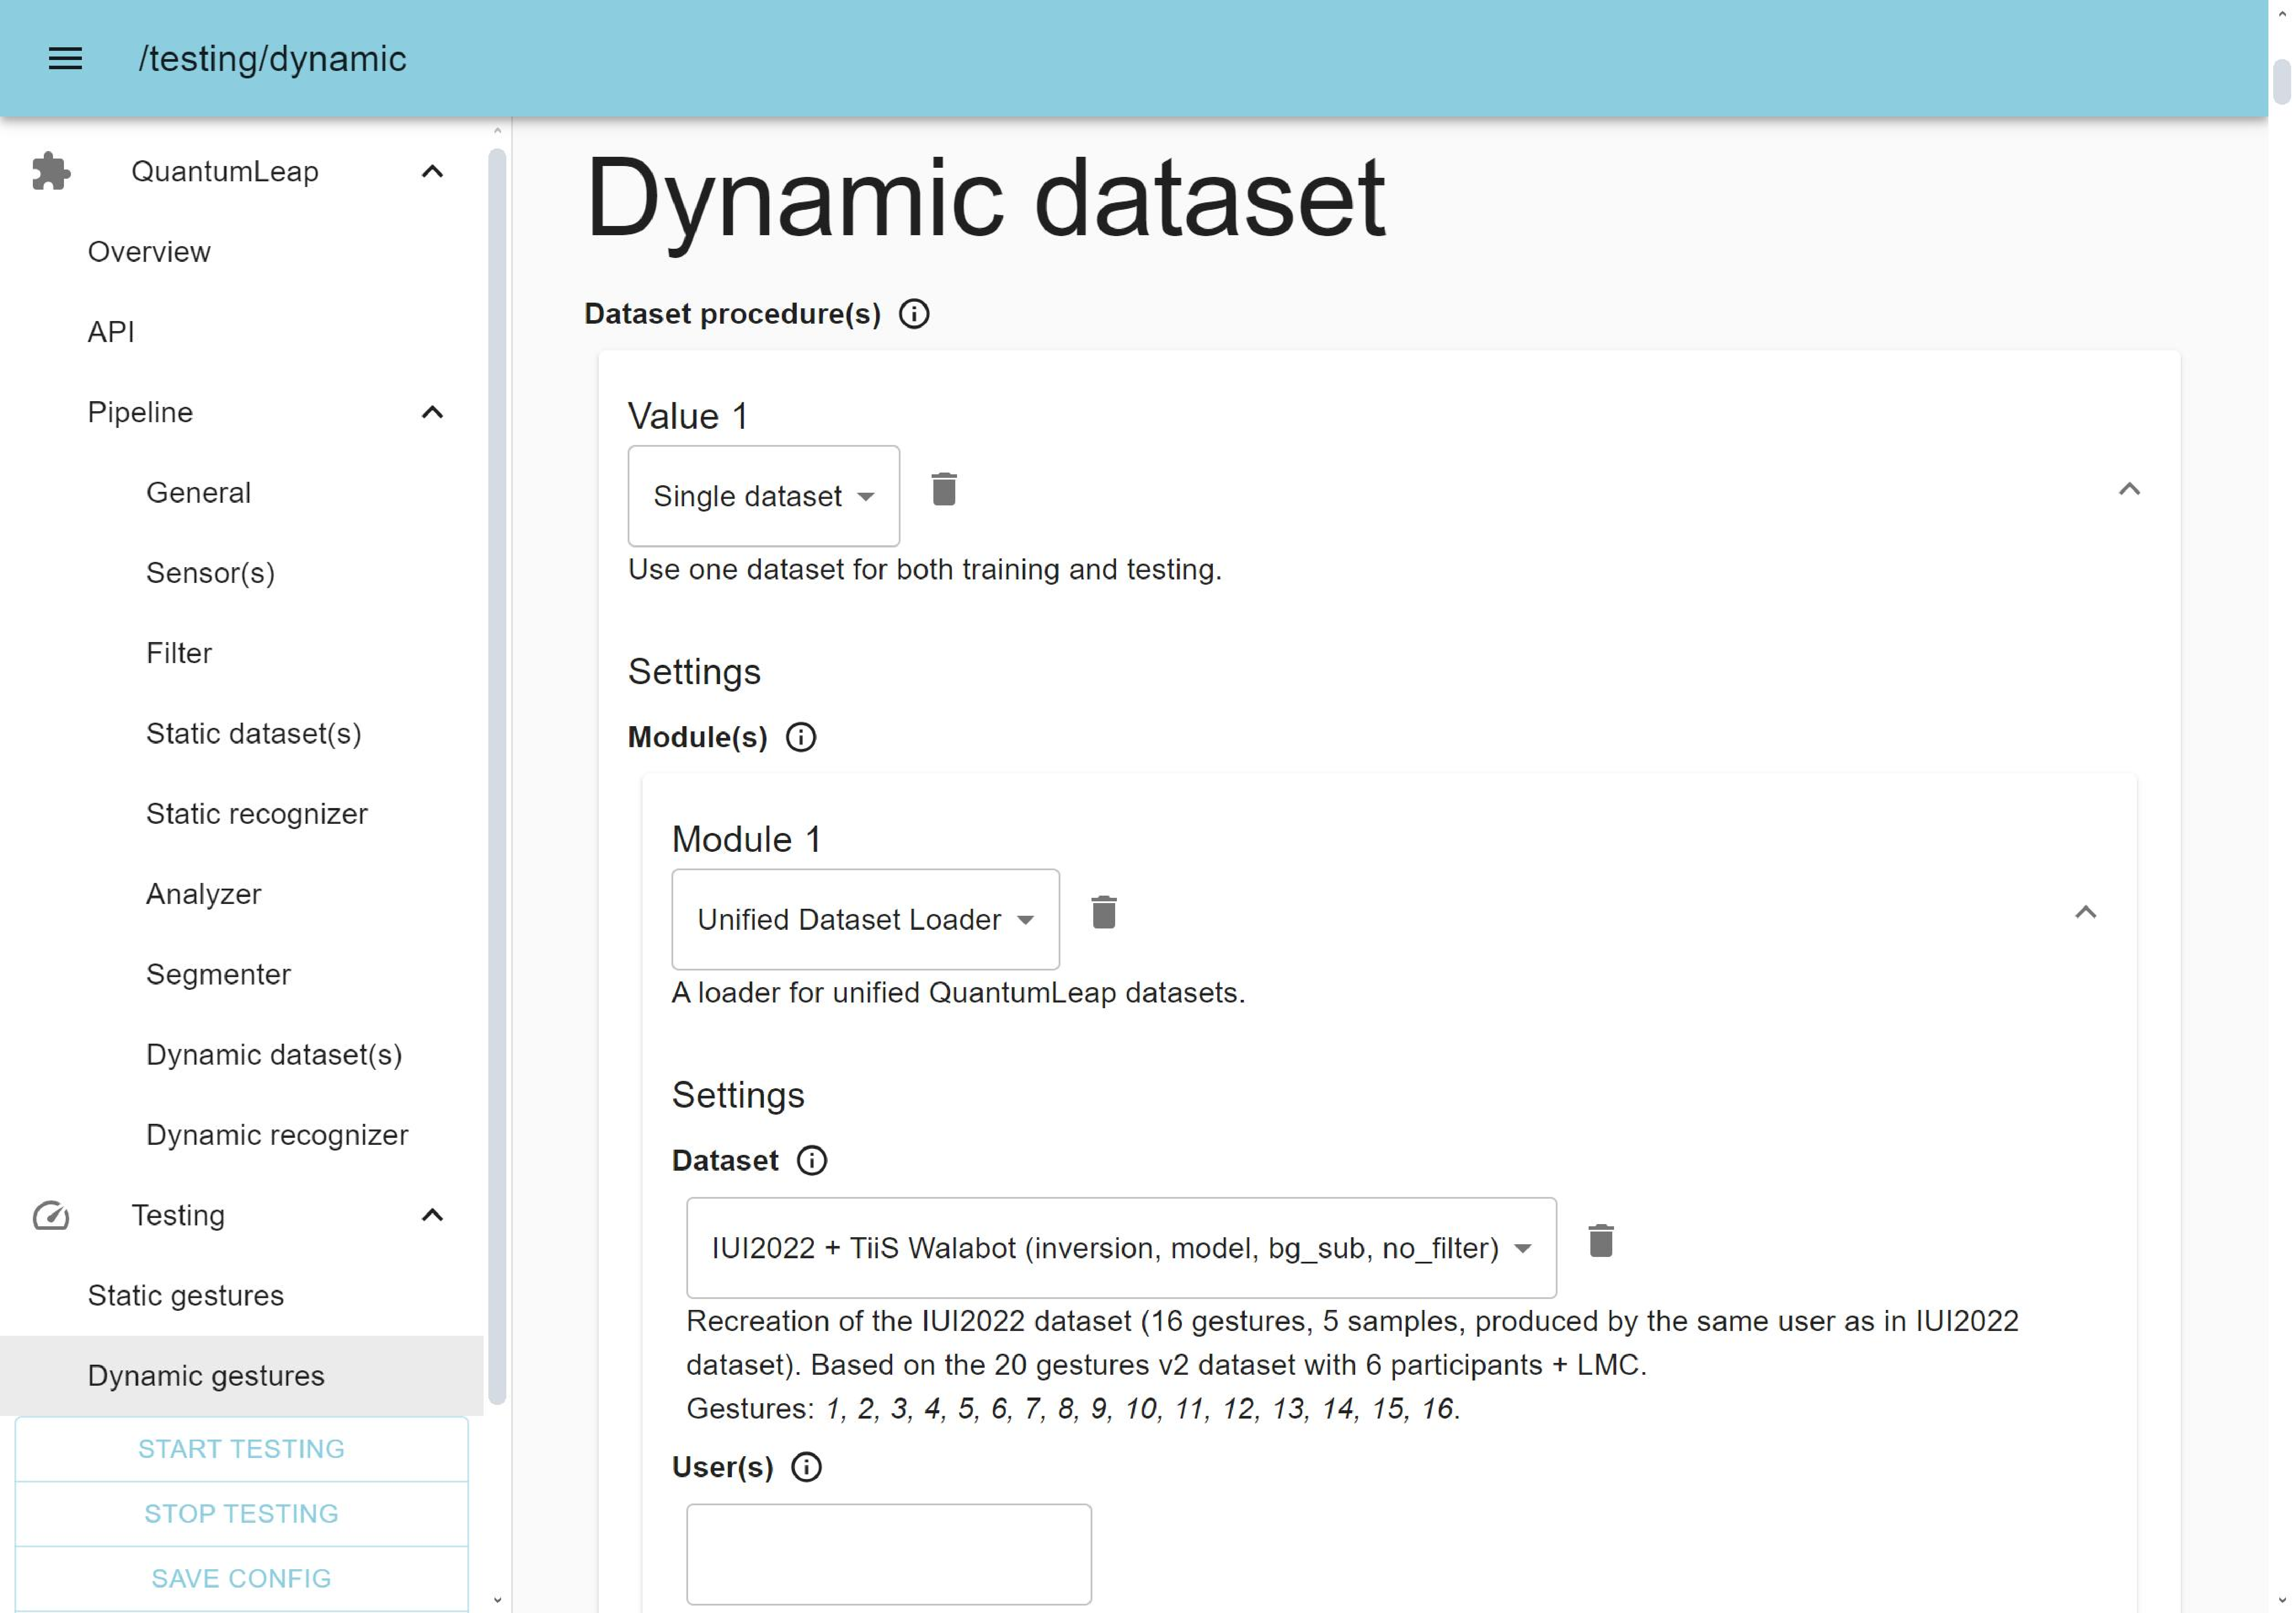
\includegraphics[width=\linewidth]{Figures/QuantumLeapTesting/QL-Testing-Dataset.pdf}  
      \vspace{-15pt}
      \captionsetup{width=.9\linewidth}
      \caption{Datasets.}
      \label{fig:quantumleap-testing:ui:2}
  \end{subfigure}
  
  \begin{subfigure}{.49\textwidth}
      \centering
      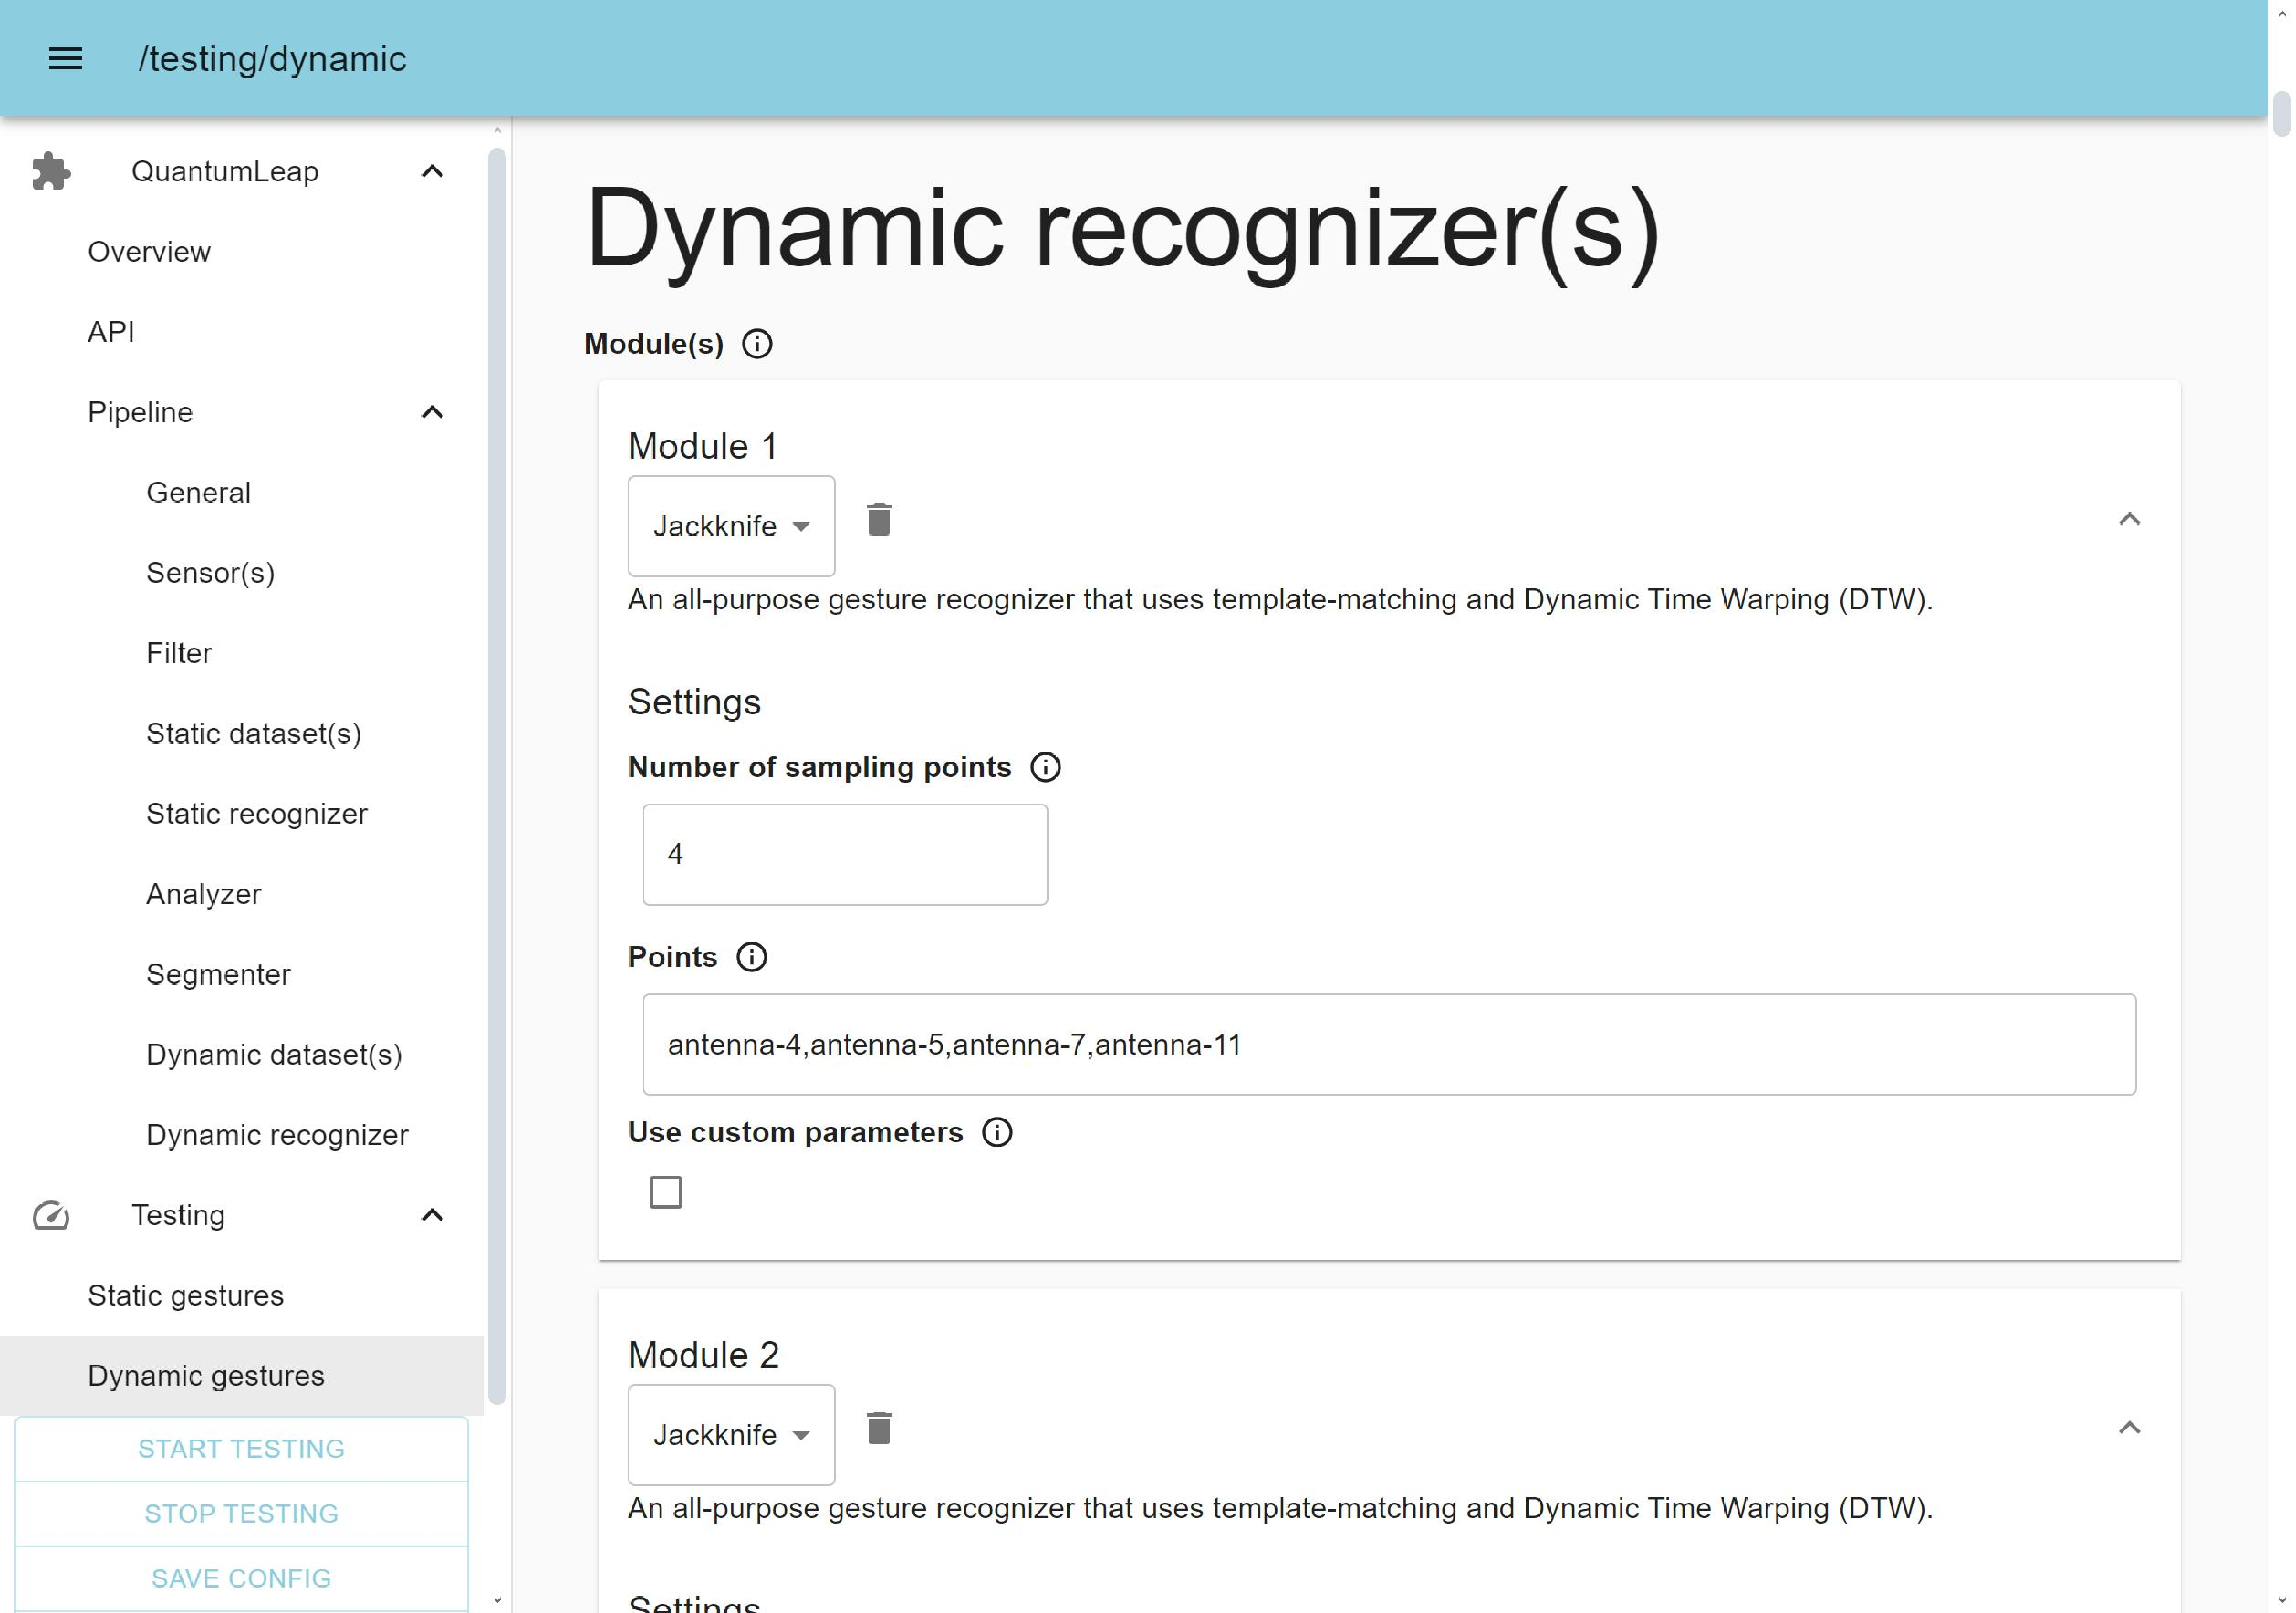
\includegraphics[width=\linewidth]{Figures/QuantumLeapTesting/QL-Testing-Recognizers.pdf}  
      \vspace{-15pt}
      \captionsetup{width=.9\linewidth}
      \caption{Recognizers.}
      \label{fig:quantumleap-testing:ui:3}
  \end{subfigure}

  % \vspace{-8pt}
  \caption{Screenshots of the \ql UI for testing.}
  \label{fig:quantumleap-testing:ui}
  % \vspace{-12pt}
\end{figure}

The testing configuration was integrated into the \ql configuration UI and features two pages: one for dynamic recognizers and another for static recognizers testing. For each type of recognizer, users can select and configure the evaluation technique(s), dataset(s), and recognizer(s) to test (\fig~\ref{fig:quantumleap-testing:ui}).
%
Testing parameters are displayed dynamically based on the ``config-template.json'' files of the testing and of any selected module. Their assigned values are read from and saved to the ``config.json'' file of the testing. This file can be easily shared with, and modified by, other users so that they can attempt to reproduce or even replicate testing results. 
%
Buttons allow users to save the configuration and start the testing. The testing status (progress, time remaining), as well as potential warnings and errors, are displayed in the terminal. 

\subsubsection{Results} \label{sec:quantumleap-testing:description:ql-integration:results}
The \textit{recognition rate} (\ie the ratio of correctly recognized gestures divided by the number of trials) and the \textit{execution time} (\ie the time for recognizing the class of a candidate gesture) are computed for each tested recognizer configuration. In addition, individual trial results are summarized in a \textit{confusion matrix} (\ie a matrix representation of the predictions from the recognizer). 
Testing results are exported to JSON files, which can be parsed manually or with specialized tools to extract data and generate graphical representations. Each file features global testing parameters (\eg number of repetitions per gesture class, evaluation technique, dataset procedure) and aggregate results for each tested recognizer configuration (recognition rate, execution time, and confusion matrix). The format of the results is described below:

\begin{customcodeblock}[]{json}
[
  {
    "r": 100,
    "evaluationTechnique": "LOOCV"
    "datasetProcedure": "singleDataset|crossDataset",
    "userScenario": "userDependent"
    "datasets": [
      "Training dataset", 
      "Testing dataset (if crossDataset)"
    ],
    "gestures": ["Gesture 1", "Gesture 2"],
    "data": [
      {
        "name": "Name of the recognizer",
        "options": {
          "Option 1": "Value",
          "Option 2": "Value"
        },
        "data": [
          {
            "accuracy": 0.375,
            "time": 10.0,
            "confusionMatrix": [
              [50 50],
              [75 25]
            ]
          }
        ]
      }
    ]
  }
]
\end{customcodeblock}

%--------------------------------------------------------------------------------%
\subsection{Testing procedures} \label{sec:quantumleap-testing:description:testing-procedures}
\ql features ten different testing procedures for evaluating the performance of gesture recognizers. Support for new procedures may be added relatively easily in the future should the need arise. The ten currently supported procedures are listed in \tab~\ref{tab:quantumleap-testing:testing-procedures} along with a detailed description. 

\begin{table}
  \footnotesize
  \centering
  \begin{tabular}{lllp{6.9cm}}
      \toprule
      \textbf{Technique} & \textbf{Users} & \textbf{Dataset(s)} & \textbf{Procedure description}\newline For each combination of independent variables [...] \\
      \midrule
      TTS     & UD    & Single & For each gesture class in the dataset, repeat $R$ times: (1) select a random sample of that class for testing, (2) train the recognizer with $N$ samples per class randomly selected from the same user, and (3) attempt recognition.\\
                      \cmidrule{3-4}
              &       & Cross  & For each gesture class in the testing set, repeat $R$ times: (1) select a random sample of that class for testing, (2) train the recognizer with $N$ samples per class randomly selected from the same user in the training set, and (3) attempt recognition. \\
              \cmidrule{2-4}
              & UI    & Single & For each gesture class in the dataset, repeat $R$ times: (1) select a random sample of that class for testing, (2) train the recognizer with $N$ samples per class randomly selected from different users than the user of the testing samples, and (3) attempt recognition.\\
                      \cmidrule{3-4}
              &       & Cross  & For each gesture class in the testing set, repeat $R$ times: (1) select a random sample of that class for testing, (2) train the recognizer with $N$ samples per class randomly selected from different users than the user of the testing samples in the training set, and (3) attempt recognition.\\
      \midrule
      LOOCV   & UD    & Single & For each gesture sample in the dataset: (1) select the sample for testing, (2) use all other samples from the same user for training, and (3) attempt recognition. \\
                      \cmidrule{3-4}
              &       & Cross  & For each gesture sample in the testing set: (1) select the sample for testing, (2) train the recognizer with all samples in the training set from the same user, and (3) attempt recognition.\\
              \cmidrule{2-4}
              & UI    & Single & For each gesture sample in the dataset: (1) select the sample for testing, (2) train the recognizer with all other samples from other users, and (3) attempt recognition. \\
                      \cmidrule{3-4}
              &       & Cross  & For each gesture sample in the testing set: (1) select the sample for testing, (2) train the recognizer with all samples in the training set from other users, and (3) attempt recognition. \\
              \cmidrule{2-4}
              & Mixed & Single & For each gesture sample in the dataset: (1) select the sample for testing, 2) train the recognizer with all other samples, and (3) attempt recognition. \\
                      \cmidrule{3-4}
              &       & Cross & For each gesture sample in the testing dataset: (1) select the sample for testing, (2) train the recognizer with all samples in the training set, and (3) attempt recognition. \\
      \bottomrule
  \end{tabular}
  \caption{Testing procedures implemented in \ql.}
  \label{tab:quantumleap-testing:testing-procedures}
\end{table}

\subsubsection{Evaluation Techniques} \label{sec:quantumleap-testing:description:testing-procedures:evaluation-techniques}
\ql supports two evaluation techniques: 
(1) train-test split (TTS), in which testing and training samples are randomly selected from the dataset(s) and 
(2) leave-one-out cross-validation (LOOCV), an extreme case of k-fold cross-validation (with $k{=}1$) in which recognizers are systematically tested with each sample of the testing dataset while training with all other valid samples of the training dataset~\cite{Zhou:2019}.

\subsubsection{Dataset Procedures} \label{sec:quantumleap-testing:description:testing-procedures:dataset-procedures}
Two dataset procedures are also supported: (1) single-dataset, in which training and testing samples are selected from the same dataset, and (2) cross-dataset, where one dataset is used for training and the other for testing. 

\subsubsection{User Scenarios} \label{sec:quantumleap-testing:description:testing-procedures:user-scenarios}
Three user scenarios are supported by \ql: (1) user-dependent (UD), in which testing and training samples are produced by the same user~\cite{Vatavu:2013}, (2) user-independent (UI), in which the testing sample is produced by a different user than the training samples~\cite{Vatavu:2013}, and (3) mixed, in which testing and training samples may or may not be produced by the same user. The UD and UI scenarios are supported by both TTS and LOOCV, while only LOOCV supports the ``mixed'' scenario.


%================================================================================%
\section{Discussion} \label{sec:quantumleap-testing:discussion}
\subsection{Strengths} \label{sec:quantumleap-testing:discussion:strengths}
The \ql testing tool has multiple advantages over using custom, opportunistic scripts for evaluating gesture recognition algorithms.
%
It allows developers and practitioners to use the same modules in an evaluation and in a final application, which is more efficient and reduces the risk of errors when switching from testing to implementation.
%
It also proposes ten predefined evaluation protocols and saves the results in a standard format, that can be parsed to produce figures and extract relevant measures.
%
Its GUI enables users to select one or more modules to evaluate and to configure them without having to modify their source code. Comparing the performance of multiple gesture recognizers in the same scenario thus becomes a painless and extremely efficient process.
%
Modules, testing configurations, and results can be shared with other researchers, providing them with all the necessary tools to attempt to repeat, replicate, and reproduce these results. By encouraging cooperation between researchers, this tool could foster the development of better algorithms for gesture recognition.

\subsection{Limitations} \label{sec:quantumleap-testing:discussion:limitations}
However, this testing tool suffers from a few limitations which could be addressed in the future.
%
For instance, evaluating a more complex gesture recognition pipeline (\eg a combination of filter, segmenter, and recognizer), while very relevant, is currently impossible without modifying the source code of the tool.
%
In addition, this tool is aimed at evaluating template-matching algorithms written in JavaScript. This currently limits its impact on the HCI community, although supporting more languages and other types of gesture recognition algorithms (\eg based on deep learning) may be possible in the future.
%
Finally, testing results are aggregated before being exported to a file, with no way to access individual trials. While these aggregated results may be easier to parse, they may not provide sufficient granularity for more in-depth analyses.

%================================================================================%
\section{Conclusion} \label{sec:quantumleap-testing:conclusion}
% Summary
In this chapter, we introduced the \ql testing tool, an extension of \ql (Chapter~\ref{chap:quantumleap}) that utilizes the same modules and datasets for evaluating the performance of gesture recognizers. It supports ten testing procedures and features standardized configuration files and results, allowing researchers to share all of the elements required to repeat, replicate, and reproduce their experiments.

% Software quality properties
Like \ql, this tool addresses the four software quality properties~\cite{iso25010} mentioned in Section~\ref{sec:introduction:research:research-questions}: compatibility, maintainability, portability, and usability.
%
As mentioned in Section~\ref{sec:quantumleap:conclusion}, \ql and its testing tool support the \textit{compatibility} property by relying on the same modules and datasets.
%
In terms of \textit{maintainability}, the \ql testing tool helps developers adapt their applications to different environments (sensor, gesture set), by making it easy to compare gesture recognizers and select the most suitable one for a specific environment.
%
Regarding \textit{portability}, \ql testing configurations, modules, and datasets can be shared by researchers so that other algorithms can be evaluated in the same conditions, thus contributing to the advancement of research on gesture recognition techniques. In addition, a testing procedure can be applied to many different modules in a matter of seconds without any modification to the source code.
%
With regards to \textit{usability}, the ability to evaluate and compare modules before employing them in an application enables developers to build more accurate gesture recognition, which can result in more usable applications.
%
Overall, our extensive use of the tool throughout the rest of this thesis highlights the benefits of designing software that satisfies these quality properties.

% Future works
Despite its advantages, the \ql testing tool still has limitations that could be addressed in future work.
%
One avenue for improvement involves supporting the evaluation of more complex gesture recognition dataflows, beyond gesture recognizers, such as combinations of filters, segmenters, and recognizers.
%
In addition, we could work on improving the granularity of the results output by the tool, to enable more in-depth analyses.
%
Finally, supporting other languages than JavaScript would vastly expand the possibilities of the tool, \eg by allowing researchers to evaluate deep learning algorithms written in Python or R.

